% !TeX root = ../documento.tex
\chapter{Metodologia Específica: Controle Digital Para um Sistema de Freio}
\label{cap:controle}

% Neste capítulo apresenta-se a metodologia específica adotada para o projeto e a avaliação de uma estratégia de controle digital aplicada ao sistema de freio, com foco na implementação de estratégias de frenagem ativa baseadas em modulação de pressão. A partir dessa estratégia, torna-se possível ajustar a força de frenagem de forma automatizada, viabilizando, entre outras aplicações, a manutenção de distância longitudinal entre veículos em arquiteturas que empregam tecnologias de assistência avançada ao condutor (ADAS), tais como o Controle de Cruzeiro Adaptativo (ACC).

% O objetivo central consiste em utilizar o módulo hidráulico de uma unidade ABS/ESC como \emph{atuador de pressão} do freio de serviço, de modo a permitir a modulação contínua da força de frenagem a partir de sinais de referência de desaceleração. Em veículos dotados de sistemas ADAS, tais referências podem ser fornecidas, por exemplo, por um controlador de distância longitudinal implementado no domínio veicular, enquanto o subsistema aqui estudado se encarrega de converter tais referências em perfis de pressão no circuito de freio.

% O Controle de Cruzeiro Adaptativo (ACC) tem sido amplamente explorado em veículos modernos como uma tecnologia de suporte à condução, cuja função principal é ajustar automaticamente a velocidade do veículo para manter uma separação segura em relação ao veículo à frente. Embora esse contexto motive o presente estudo, o escopo deste trabalho está concentrado no subsistema de freio: em particular, na modelagem e no controle do bloco hidráulico composto por bomba, válvulas solenóide e volumes equivalentes de fluido, que realiza a geração e a modulação da pressão de frenagem.

% Apesar da extensa literatura em estratégias de frenagem ativa e controle longitudinal, observa-se que muitos trabalhos permanecem restritos a simulações em alto nível, com abstrações simplificadas do atuador de freio. Abordagens que integram explicitamente a dinâmica hidráulica da unidade ABS/ESC ao projeto de controle ainda são relativamente menos exploradas, sobretudo no que se refere à implementação em arquiteturas digitais e à análise detalhada da dinâmica de pressurização e despressurização \cite{HouhuaJing2022,PressureCoordinatedControl2023}. Este trabalho busca contribuir nesse sentido, adotando uma formulação em espaço de estados que incorpora tanto a dinâmica longitudinal do veículo quanto o comportamento do subsistema hidráulico de freio.

% A metodologia proposta segue a filosofia de integração entre subsistemas de controle veicular e atuadores de frenagem observada em trabalhos sobre sistemas de freio eletro-hidráulicos e integrados \cite{HouhuaJing2022,PressureCoordinatedControl2023,MotorParametricDesign2023}. Em particular, emprega-se um modelo em espaço de estados da planta (veículo mais subsistema hidráulico de freio) para o projeto de um controlador em espaço de estados, implementado digitalmente, o qual gera sinais de comando para as válvulas e para a bomba da unidade hidráulica.

% De forma resumida, a metodologia adotada neste capítulo pode ser organizada nas seguintes etapas:

% \begin{enumerate}
%     \item \textbf{Modelagem da planta em espaço de estados}: a partir de um modelo de dinâmica longitudinal do veículo e de um modelo concentrado do subsistema hidráulico de freio, obtém-se uma representação em espaço de estados adequada ao projeto de controladores lineares. Essa representação incorpora explicitamente a pressão no circuito de freio como variável de estado relevante para a geração da força de frenagem.

%     \item \textbf{Integração com atuadores hidráulicos}: o módulo hidráulico ABS/ESC é modelado como um atuador de pressão composto por bomba, válvulas solenóide de entrada e saída e volumes equivalentes de fluido, seguindo a abordagem de unidades hidráulicas utilizadas em sistemas ESC e EHB \cite{ZengYangHuang2023,HouhuaJing2022}. Essa integração permite relacionar diretamente os sinais de controle digitais (por exemplo, ciclos de trabalho PWM) aos perfis de pressão no canal das rodas, aproximando o modelo de configurações empregadas em unidades hidráulicas reais.

%     \item \textbf{Discretização e implementação digital}: o modelo contínuo da planta é discretizado considerando o período de amostragem disponível na unidade eletrônica de controle, o que viabiliza a síntese de um controlador digital em espaço de estados (por exemplo, um regulador linear quadrático em tempo discreto) compatível com a arquitetura de controle embarcada.

%     \item \textbf{Validação em simulação}: por meio de simulações em MATLAB/Simulink, são avaliadas a resposta de pressão no freio e a resposta longitudinal do veículo sob diferentes comandos de frenagem ativa e perturbações, em linha com metodologias de validação de sistemas de freio eletro-hidráulicos reportadas na literatura \cite{ZengYangHuang2023,MotorParametricDesign2023}. Nessa etapa, são realizados ensaios em malha aberta para validação do modelo hidráulico, seguidos de ensaios em malha fechada com o controlador digital projetado.
% \end{enumerate}

% Diferentemente de abordagens que fazem uso direto de atuadores eletromecânicos de freio de estacionamento eletrônico (EPB) como elemento de \textit{backup} para geração de força de frenagem \cite{HouhuaJingShihao2023}, o presente trabalho concentra-se no uso do módulo hidráulico do ABS/ESC como atuador principal de pressão para o freio de serviço. Essa escolha permite explorar a infraestrutura hidráulica já disponível no veículo, ao mesmo tempo em que exige uma modelagem cuidadosa da dinâmica de pressurização e despressurização do circuito de freio, que será detalhada nas seções subsequentes.

% ####################################################
% ####################################################
% ####################################################

% Neste capítulo apresenta-se a metodologia específica adotada para o projeto e a avaliação de uma estratégia de controle digital aplicada ao sistema de freio, com foco na implementação de estratégias de frenagem ativa baseadas em modulação de pressão. A partir dessa estratégia, torna-se possível ajustar a força de frenagem de forma automatizada, viabilizando, entre outras aplicações, o atendimento a referências de desaceleração provenientes de sistemas de assistência avançada ao condutor (ADAS), tais como o Controle de Cruzeiro Adaptativo (ACC).

% O objetivo central consiste em utilizar o módulo hidráulico de uma unidade ABS/ESC como \emph{atuador de pressão} do freio de serviço, de modo a permitir a modulação contínua da força de frenagem a partir de sinais de referência de desaceleração. Em arquiteturas veiculares dotadas de sistemas ADAS, tais referências podem ser fornecidas, por exemplo, por um controlador de distância longitudinal implementado em um nível superior de controle, enquanto o subsistema aqui estudado se encarrega de converter essas referências em perfis de pressão no circuito de freio.

% Nesse contexto, o ACC e a distância longitudinal desempenham o papel de fontes externas de referência: assume-se que um módulo de controle longitudinal fornece um sinal de aceleração desejada $a_{\mathrm{ego}}(t)$, o qual é convertido em uma pressão de referência $P_{\mathrm{ref}}(t)$ por meio de relações estáticas entre desaceleração, força de frenagem e pressão hidráulica no cáliper. Um exemplo simplificado dessa conversão, utilizado nas simulações, é dado por
% \[
%     F_{\mathrm{freno}} = m\,|a_{\mathrm{ego}}|, 
%     \qquad
%     P_{\mathrm{ref}} = \frac{F_{\mathrm{freno}}}{A_{cal}},
% \]
% em que $m$ é a massa equivalente do veículo e $A_{cal}$ é a área efetiva do pistão do cáliper. A partir de $P_{\mathrm{ref}}(t)$, o problema tratado neste trabalho reduz-se ao controle da pressão no canal da roda $P_w(t)$, utilizando o módulo hidráulico ABS/ESC como atuador.

% Apesar da extensa literatura em estratégias de frenagem ativa e controle longitudinal, observa-se que muitos trabalhos permanecem restritos a simulações em alto nível, com abstrações simplificadas do atuador de freio. Abordagens que integram explicitamente a dinâmica hidráulica da unidade ABS/ESC ao projeto de controladores de pressão ainda são relativamente menos exploradas, sobretudo no que se refere à implementação em arquiteturas digitais e à análise detalhada da dinâmica de pressurização e despressurização \cite{HouhuaJing2022,PressureCoordinatedControl2023}. Este trabalho busca contribuir nesse sentido, adotando uma formulação em espaço de estados para o subsistema hidráulico de freio e investigando o desempenho de controladores digitais de pressão.

% A metodologia proposta segue a filosofia de integração entre subsistemas de controle veicular e atuadores de frenagem observada em trabalhos sobre sistemas de freio eletro-hidráulicos e integrados \cite{HouhuaJing2022,PressureCoordinatedControl2023,MotorParametricDesign2023}. Em particular, emprega-se um modelo em espaço de estados do atuador hidráulico de freio para o projeto de um controlador em espaço de estados, implementado digitalmente, o qual gera sinais de comando para as válvulas e para a bomba da unidade hidráulica de modo a rastrear $P_{\mathrm{ref}}(t)$.

% De forma resumida, a metodologia adotada neste capítulo pode ser organizada nas seguintes etapas:

% \begin{enumerate}
%     \item \textbf{Modelagem do atuador hidráulico em espaço de estados}: a partir de um modelo concentrado do subsistema hidráulico de freio (bomba, válvulas e volumes equivalentes), obtém-se uma representação em espaço de estados adequada ao projeto de controladores lineares de pressão.

%     \item \textbf{Integração com sinais de referência externos}: o módulo hidráulico ABS/ESC é utilizado como elemento de atuação que recebe, como entrada de referência, um sinal de pressão $P_{\mathrm{ref}}(t)$ derivado de requisitos de desaceleração $a_{\mathrm{ego}}(t)$ fornecidos por sistemas de controle longitudinal em nível superior.

%     \item \textbf{Discretização e implementação digital}: o modelo contínuo do atuador hidráulico é discretizado considerando o período de amostragem disponível na unidade eletrônica de controle, o que viabiliza a síntese de um controlador digital em espaço de estados (por exemplo, um regulador linear quadrático em tempo discreto) compatível com a arquitetura de controle embarcada.

%     \item \textbf{Validação em simulação}: por meio de simulações em MATLAB/Simulink, é avaliado o rastreamento da pressão no freio frente a diferentes perfis de $P_{\mathrm{ref}}(t)$ e perturbações, em linha com metodologias de validação de sistemas de freio eletro-hidráulicos reportadas na literatura \cite{ZengYangHuang2023,MotorParametricDesign2023}. Nessa etapa, são realizados ensaios em malha aberta para validação do modelo hidráulico, seguidos de ensaios em malha fechada com o controlador digital projetado.
% \end{enumerate}

% Diferentemente de abordagens que fazem uso direto de atuadores eletromecânicos de freio de estacionamento eletrônico (EPB) como elemento de backup para geração de força de frenagem \cite{HouhuaJingShihao2023}, o presente trabalho concentra-se no uso do módulo hidráulico do ABS/ESC como atuador principal de pressão para o freio de serviço. Essa escolha permite explorar a infraestrutura hidráulica já disponível no veículo, ao mesmo tempo em que exige uma modelagem cuidadosa da dinâmica de pressurização e despressurização do circuito de freio, que será detalhada nas seções subsequentes.

Neste capítulo apresenta-se a metodologia específica adotada para o projeto e a avaliação de uma estratégia de controle digital aplicada ao sistema de freio, com foco na implementação de estratégias de frenagem ativa baseadas em modulação de pressão. A partir dessa estratégia, torna-se possível ajustar a força de frenagem de forma automatizada, viabilizando, entre outras aplicações, o atendimento a referências de desaceleração provenientes de sistemas de assistência avançada ao condutor (ADAS), tais como o Controle de Cruzeiro Adaptativo (ACC).

O objetivo central consiste em utilizar o módulo hidráulico de uma unidade ABS/ESC como \emph{atuador de pressão} do freio de serviço, de modo a permitir a modulação contínua da força de frenagem a partir de sinais de referência de desaceleração. Em arquiteturas veiculares dotadas de sistemas ADAS, tais referências podem ser fornecidas, por exemplo, por um controlador de distância longitudinal implementado em um nível superior de controle, enquanto o subsistema aqui estudado se encarrega de converter essas referências em perfis de pressão no circuito de freio.

Nesse contexto, o ACC e a distância longitudinal desempenham o papel de fontes externas de referência: assume-se que um módulo de controle longitudinal fornece um sinal de desaceleração desejada $a_{\mathrm{ego}}(t)$, o qual é convertido em uma pressão de referência $P_{\mathrm{ref}}(t)$ por meio de relações estáticas entre desaceleração, força de frenagem e pressão hidráulica no cáliper. Um exemplo simplificado dessa conversão, utilizado nas simulações, é dado por
\[
    F_{\mathrm{freno}} = m\,|a_{\mathrm{ego}}|, 
    \qquad
    P_{\mathrm{ref}} = \frac{F_{\mathrm{freno}}}{A_{cal}},
\]
em que $m$ é a massa equivalente do veículo e $A_{cal}$ é a área efetiva do pistão do cáliper. A partir de $P_{\mathrm{ref}}(t)$, o problema tratado neste trabalho reduz-se ao controle da pressão no canal da roda $P_w(t)$, utilizando o módulo hidráulico ABS/ESC como atuador.

Embora exista uma literatura extensa em estratégias de frenagem ativa e controle longitudinal, observa-se que muitos trabalhos permanecem restritos a simulações em alto nível, com abstrações simplificadas do atuador de freio. Abordagens que integram explicitamente a dinâmica hidráulica da unidade ABS/ESC ao projeto de controladores de pressão ainda são relativamente menos exploradas, sobretudo no que se refere à implementação em arquiteturas digitais e à análise detalhada da dinâmica de pressurização e despressurização \cite{HouhuaJing2022,PressureCoordinatedControl2023}. Este trabalho busca contribuir nesse sentido, adotando uma formulação em espaço de estados para o subsistema hidráulico de freio e investigando o desempenho de controladores digitais de pressão.

A metodologia proposta segue a filosofia de integração entre subsistemas de controle veicular e atuadores de frenagem observada em trabalhos sobre sistemas de freio eletro-hidráulicos e integrados \cite{HouhuaJing2022,PressureCoordinatedControl2023,MotorParametricDesign2023}. Em particular, emprega-se um modelo em espaço de estados do atuador hidráulico de freio para o projeto de um controlador em espaço de estados, implementado digitalmente, o qual gera sinais de comando para as válvulas e para a bomba da unidade hidráulica de modo a rastrear $P_{\mathrm{ref}}(t)$.

De forma resumida, a metodologia adotada neste capítulo pode ser organizada nas seguintes etapas:

\begin{enumerate}
    \item \textbf{Modelagem do atuador hidráulico em espaço de estados}: a partir de um modelo concentrado do subsistema hidráulico de freio (bomba, válvulas e volumes equivalentes), obtém-se uma representação em espaço de estados adequada ao projeto de controladores lineares de pressão.

    \item \textbf{Integração com sinais de referência externos}: o módulo hidráulico ABS/ESC é utilizado como elemento de atuação que recebe, como entrada de referência, um sinal de pressão $P_{\mathrm{ref}}(t)$ derivado de requisitos de desaceleração $a_{\mathrm{ego}}(t)$ fornecidos por sistemas de controle longitudinal em nível superior.

    \item \textbf{Discretização e implementação digital}: o modelo contínuo do atuador hidráulico é discretizado considerando o período de amostragem disponível na unidade eletrônica de controle, o que viabiliza a síntese de um controlador digital em espaço de estados (por exemplo, um regulador linear quadrático em tempo discreto com observador de Luenberger) compatível com a arquitetura de controle embarcada.

    \item \textbf{Validação em simulação}: por meio de simulações em MATLAB/Simulink, é avaliado o rastreamento da pressão no freio frente a diferentes perfis de $P_{\mathrm{ref}}(t)$ e perturbações, em linha com metodologias de validação de sistemas de freio eletro-hidráulicos reportadas na literatura \cite{ZengYangHuang2023,MotorParametricDesign2023}. Nessa etapa, são realizados ensaios em malha aberta para validação do modelo hidráulico, seguidos de ensaios em malha fechada com o controlador digital projetado.
\end{enumerate}

Diferentemente de abordagens que fazem uso direto de atuadores eletromecânicos de freio de estacionamento eletrônico (EPB) como elemento de backup para geração de força de frenagem \cite{HouhuaJingShihao2023}, o presente trabalho concentra-se no uso do módulo hidráulico do ABS/ESC como atuador principal de pressão para o freio de serviço. Essa escolha permite explorar a infraestrutura hidráulica já disponível no veículo, ao mesmo tempo em que exige uma modelagem cuidadosa da dinâmica de pressurização e despressurização do circuito de freio, que será detalhada nas seções subsequentes.


%####################################################################
%####################################################################
%####################################################################
%####################################################################
\section{Modelagem da Planta}
\label{sec:controle-4-1}

% O objetivo desta seção é apresentar a modelagem da planta do sistema de frenagem, com ênfase na atuação da placa de controle digital sobre os componentes do módulo hidráulico — especificamente, as válvulas solenoides e a bomba de pressão. O comportamento do sistema ACC é utilizado como cenário de aplicação, mas o foco principal está na implementação prática do controle embarcado.

% Em veículos modernos, a arquitetura \textit{brake-by-wire} (freio por fio) e a substituição de conexões mecânicas por atuadores eletrônicos têm possibilitado maior integração com sistemas de controle embarcados. Essa abordagem é relevante para a implementação de estratégias de frenagem ativa, como o ACC, e tem sido objeto de investigação em veículos experimentais \cite{Pananurak2009}.

% Neste trabalho, optou-se por uma modelagem simplificada da dinâmica longitudinal do veículo, suficiente para validar a estratégia de controle digital proposta e a atuação da placa desenvolvida. Embora existam modelos mais completos na literatura, que incluem motor, conversor de torque, transmissão e rodas \cite{LuuAndLupu2019}, tais abordagens demandam maior complexidade computacional e não constituem o foco deste estudo.

% Adota-se um contexto longitudinal simplificado apenas para gerar referências de desaceleração/frenagem; a validação desta etapa concentra-se na coerência física do subsistema hidráulico em malha aberta.

% A arquitetura hierárquica do ACC pode ser dividida em dois níveis: um controlador de alto nível, responsável por calcular a aceleração desejada (por exemplo, via \textit{Model Predictive Control} - MPC), e um controlador de baixo nível, que executa os comandos nos atuadores. Essa estrutura, conforme descrito por \citeonline{Tian2024}, pode contribuir para a estabilidade e segurança do sistema em tempo real.

% Para representar a lógica de comutação entre acelerador e freio, abordagens como a modelagem \textit{Mixed Logical Dynamical} (MLD) são utilizadas na literatura \cite{LihuaLuo2016}, permitindo capturar o comportamento híbrido do sistema ACC. No entanto, neste estudo, adota-se uma modelagem contínua simplificada, considerada suficiente para os objetivos de validação da estratégia de controle digital e da placa desenvolvida.

% No contexto do sistema de frenagem, a precisão na modulação da pressão hidráulica é um aspecto central. Pesquisas como a de \citeonline{ChenLv2017} propõem o uso de válvulas de comutação com controle linear da queda de pressão, enquanto \citeonline{HouhuaJing2022} destaca o uso de válvulas do tipo \textit{High-Speed Valve} (HSV) e \textit{Unload Solenoid Valve} (USV), controladas por modulação por largura de pulso (PWM) para ajuste da pressão nos cilindros das rodas. Recentemente, métodos de controle coordenado de pressão foram propostos para sistemas eletro-hidráulicos, visando melhorar a resposta dinâmica e a robustez do sistema de freio, conforme apresentado em \citeonline{PressureCoordinatedControl2023} e \citeonline{ProportionalPressureABS2023}.

% Dessa forma, a modelagem adotada neste projeto considera a dinâmica longitudinal do veículo, com ênfase na atuação da placa de controle sobre os atuadores hidráulicos. A placa desenvolvida é responsável por gerar sinais para controlar as válvulas, além de acionar a bomba de pressão. Essa arquitetura permite modular a pressão de frenagem de maneira ajustável, dentro das limitações do modelo e do ambiente experimental.

% Cabe ressaltar que, embora a modelagem proposta seja fundamentada em referências consolidadas, ela incorpora simplificações necessárias para viabilizar a implementação em ambiente embarcado e simulado. Aspectos como não linearidades complexas, variações térmicas do fluido, compressibilidade dependente da temperatura e atrasos eletromecânicos dos atuadores não são explicitamente considerados neste estágio. Tais efeitos, reconhecidos na literatura como mais significativos para a dinâmica do sistema do que a histerese individual das válvulas, são deixados para estudos futuros que possam aprofundar a análise em maior detalhe. Assim, os resultados apresentados devem ser interpretados como uma contribuição incremental para o entendimento e validação de estratégias de controle digital em sistemas de frenagem automotiva.

% #########################################################################################################

% O projeto de um controlador em espaço de estados para o sistema de freio requer uma representação dinâmica que incorpore, de forma integrada, a dinâmica longitudinal do veículo e o comportamento do subsistema hidráulico responsável pela geração da pressão de frenagem. Nesta seção, apresenta-se a modelagem da planta adotada, estruturada em torno de dois blocos principais: (i) o modelo longitudinal veicular e (ii) o modelo concentrado do atuador hidráulico de freio.

% A literatura sobre sistemas de frenagem eletro-hidráulicos e integrados evidencia a importância de modelos que representem, ainda que de forma reduzida, a interação entre o atuador de pressão e a dinâmica veicular, seja para fins de projeto de controladores, seja para validação em ambiente \emph{hardware-in-the-loop} \cite{HouhuaJing2022,PressureCoordinatedControl2023,DesignESCUnitTestSystem2018,MotorParametricDesign2023}. Trabalhos como \citeonline{HouhuaJing2022} e \citeonline{ZengYangHuang2023} empregam modelos concentrados para descrever a relação entre comandos em válvulas solenóide, pressão no cilindro da roda e força de frenagem, enquanto \citeonline{MotorParametricDesign2023} integra explicitamente o modelo da bomba acionada por motor elétrico à dinâmica hidráulica, visando à análise de desempenho sob diferentes perfis de frenagem.

% No presente trabalho, a planta é modelada a partir de um esquema em dois níveis:

% \begin{itemize}
%     \item No nível veicular, considera-se a dinâmica longitudinal em uma dimensão, relacionando a força resultante no sentido do movimento à aceleração do veículo, sob a ação de forças de tração, resistência e frenagem.

%     \item No nível de atuador, o módulo hidráulico ABS/ESC é representado por um modelo em duas pressões (suprimento e canal da roda), incluindo bomba, vazamentos internos e válvulas de entrada e saída modeladas por lei de orifício. A pressão no canal da roda é então convertida em força de frenagem equivalente sobre o veículo.
% \end{itemize}

% A seguir, descrevem-se brevemente esses dois blocos.

% \subsection{Modelo longitudinal do veículo}
% \label{sec:modelo-longitudinal}

% Adota-se um modelo de veículo concentrado em uma única massa equivalente $m$, em movimento ao longo de uma trajetória retilínea, de forma semelhante a outros estudos de controle longitudinal e de sistemas de frenagem ativa \cite{HouhuaJing2022,PressureCoordinatedControl2023}. A equação de movimento na direção longitudinal pode ser escrita como
% \begin{equation}
%     m\,\dot{v}(t) = F_{\text{trac}}(t) - F_{\text{res}}(t) - F_{\text{freno}}(t),
%     \label{eq:veiculo-longitudinal}
% \end{equation}
% em que $v(t)$ é a velocidade do veículo, $F_{\text{trac}}(t)$ representa a força de tração (quando presente), $F_{\text{res}}(t)$ agrega os esforços resistivos (aerodinâmicos, rolamento e rampa, se considerados) e $F_{\text{freno}}(t)$ é a força resultante de frenagem aplicada ao veículo.

% No contexto deste trabalho, o foco recai sobre a componente de frenagem, de modo que $F_{\text{trac}}(t)$ pode ser tratada como entrada externa ou, em cenários de frenagem pura, considerada nula. A força de frenagem é modelada a partir da pressão no circuito hidráulico e da geometria do sistema de freio (cilindro, cáliper e roda), de acordo com
% \begin{equation}
%     F_{\text{freno}}(t) = \eta_b\,\frac{P_w(t)\,A_{cal}\,R_{w}}{r_{eq}},
%     \label{eq:forca-freno-equivalente}
% \end{equation}
% em que $P_w(t)$ é a pressão no canal da roda, $A_{cal}$ é a área efetiva do pistão do cáliper, $R_{w}$ é o raio efetivo de frenagem no disco, $r_{eq}$ é o raio dinâmico equivalente da roda/trenó e $\eta_b$ é um coeficiente de eficiência global que engloba perdas mecânicas e conversão de força na interface pneu–pavimento. Relações desse tipo são comumente utilizadas em estudos que conectam modelos hidráulicos de freio à dinâmica veicular \cite{DesignESCUnitTestSystem2018,BackupEPBActuator2020}.

% \subsection{Modelo concentrado do atuador hidráulico}
% \label{sec:modelo-atuador-hidraulico}

% O subsistema hidráulico é baseado na arquitetura típica de unidades ABS/ESC, compostas por uma bomba de retorno, válvulas solenóide de entrada e saída e câmara de roda conectada ao cáliper. Para fins de projeto de controle, adota-se um modelo concentrado em duas pressões: a pressão de suprimento $P_{sup}(t)$, associada ao manifold pressurizado pela bomba, e a pressão $P_w(t)$ no canal da roda. Modelos de estrutura similar são empregados em \citeonline{HouhuaJing2022} e \citeonline{ZengYangHuang2023} para descrever a dinâmica de pressurização e despressurização em sistemas de freio eletro-hidráulicos.

% As equações de continuidade de massa para os volumes equivalentes de suprimento e de roda podem ser escritas como
% \begin{align}
%     \dot{P}_{sup}(t) &= \frac{\beta}{V_{sup}}\left(Q_{\text{pump}}(t) - Q_{in}(t) - Q_{\text{leak,sup}}(t)\right),
%     \label{eq:psup-dot}\\[4pt]
%     \dot{P}_{w}(t) &= \frac{\beta}{V_{w}}\left(Q_{in}(t) - Q_{out}(t) - Q_{\text{leak,w}}(t)\right),
%     \label{eq:pw-dot}
% \end{align}
% em que $\beta$ é o módulo volumétrico efetivo do fluido, $V_{sup}$ e $V_{w}$ são os volumes equivalentes associados ao suprimento e ao canal da roda, $Q_{\text{pump}}(t)$ é a vazão fornecida pela bomba, $Q_{in}(t)$ e $Q_{out}(t)$ são as vazões através das válvulas de entrada e saída, respectivamente, e $Q_{\text{leak,sup}}(t)$ e $Q_{\text{leak,w}}(t)$ representam vazamentos internos, quando considerados. A forma funcional de $Q_{in}(t)$ e $Q_{out}(t)$, baseada na lei de orifício, é detalhada na Seção~\ref{sec:controle-valvulas-orificio}, enquanto o modelo da bomba e dos vazamentos internos é apresentado na Seção~\ref{sec:controle-bomba-vazamento}.

% A integração entre o modelo do atuador hidráulico e o modelo longitudinal do veículo ocorre por meio da pressão $P_w(t)$, que, via \eqref{eq:forca-freno-equivalente}, determina a força de frenagem aplicada na equação de movimento \eqref{eq:veiculo-longitudinal}. A partir das equações \eqref{eq:veiculo-longitudinal}–\eqref{eq:pw-dot}, é possível organizar a planta em uma representação em espaço de estados, escolhendo-se, por exemplo, o vetor de estados
% \begin{equation}
%     x(t) = 
%     \begin{bmatrix}
%         v(t) \\
%         P_{sup}(t) \\
%         P_{w}(t)
%     \end{bmatrix},
%     \label{eq:vect-estados}
% \end{equation}
% e definindo os sinais de controle como as variáveis associadas à atuação na bomba e nas válvulas (por exemplo, a velocidade da bomba e os comandos $u_{in}$ e $u_{out}$ das válvulas solenóide). Essa estrutura em espaço de estados serve de base para o projeto do controlador digital em seções posteriores.

% A adoção de um modelo concentrado, embora simplificada em comparação com descrições distribuídas ou com modelos detalhados de dinâmica de válvulas, é coerente com abordagens empregadas em estudos de controle de pressão em HCUs automotivas \cite{HouhuaJing2022,DesignESCUnitTestSystem2018,HardwareInTheLoopPDL2014}. Tal opção permite capturar os principais efeitos dinâmicos relevantes para o controle (compressibilidade do fluido, volumes equivalentes, limitações de vazão em válvulas) com complexidade compatível com a implementação em ambientes de simulação e controle digital.

% O projeto de um controlador em espaço de estados para o sistema de freio requer uma representação dinâmica da planta que descreva, com fidelidade adequada, o comportamento do subsistema responsável pela geração e modulação da pressão de frenagem. Neste trabalho, a planta a ser controlada é o módulo hidráulico da unidade ABS/ESC, modelado como um atuador de pressão composto por bomba, válvulas solenóide e volumes equivalentes de fluido.

% Aspectos de controle longitudinal em nível veicular, como a geração de referências de aceleração a partir da distância longitudinal em relação a um veículo à frente, são tratados aqui como funcionalidades externas ao escopo deste estudo. Assume-se que um sistema de controle em nível superior fornece um sinal de desaceleração desejada $a_{\mathrm{ego}}(t)$, o qual é convertido em uma pressão de referência $P_{\mathrm{ref}}(t)$ por meio de relações estáticas entre desaceleração, força de frenagem e pressão no cáliper. A partir dessa referência, o problema abordado neste capítulo consiste em fazer com que a pressão no canal da roda $P_w(t)$ siga $P_{\mathrm{ref}}(t)$ com desempenho adequado.

% Para fins de consistência física, considera-se a relação aproximada
% \begin{equation}
%     F_{\mathrm{freno}} = m\,|a_{\mathrm{ego}}|, 
%     \qquad
%     P_{\mathrm{ref}} = \frac{F_{\mathrm{freno}}}{A_{cal}},
%     \label{eq:relacao-aego-pressao}
% \end{equation}
% em que $m$ é a massa equivalente do veículo e $A_{cal}$ é a área efetiva do pistão do cáliper. Essa relação, implementada em ambiente de simulação como uma função de conversão entre $a_{\mathrm{ego}}$ e $P_{\mathrm{ref}}$, não é incluída na dinâmica da planta controlada, mas fornece o vínculo físico entre o domínio longitudinal veicular e o domínio hidráulico do freio.

% A literatura sobre sistemas de frenagem eletro-hidráulicos e integrados evidencia a importância de modelos concentrados para descrever a relação entre comandos em válvulas solenóide, pressão no cilindro da roda e força de frenagem, seja para fins de projeto de controladores, seja para validação em ambiente \emph{hardware-in-the-loop} \cite{HouhuaJing2022,PressureCoordinatedControl2023,DesignESCUnitTestSystem2018,MotorParametricDesign2023}. Trabalhos como \citeonline{HouhuaJing2022} e \citeonline{ZengYangHuang2023} empregam modelos em duas pressões para descrever a dinâmica de pressurização e despressurização em sistemas de freio eletro-hidráulicos, enquanto \citeonline{DesignESCUnitTestSystem2018} e \citeonline{HardwareInTheLoopPDL2014} utilizam descrições semelhantes na análise experimental de unidades hidráulicas de ESC.

% No presente trabalho, o módulo hidráulico é modelado a partir de um esquema em duas pressões: a pressão de suprimento $P_{sup}(t)$, associada ao manifold pressurizado pela bomba, e a pressão $P_w(t)$ no canal da roda. As equações de continuidade de massa para os volumes equivalentes de suprimento e de roda podem ser escritas como
% \begin{align}
%     \dot{P}_{sup}(t) &= \frac{\beta}{V_{sup}}\left(Q_{\text{pump}}(t) - Q_{in}(t) - Q_{\text{leak,sup}}(t)\right),
%     \label{eq:psup-dot}\\[4pt]
%     \dot{P}_{w}(t) &= \frac{\beta}{V_{w}}\left(Q_{in}(t) - Q_{out}(t) - Q_{\text{leak,w}}(t)\right),
%     \label{eq:pw-dot}
% \end{align}
% em que $\beta$ é o módulo volumétrico efetivo do fluido, $V_{sup}$ e $V_{w}$ são os volumes equivalentes associados ao suprimento e ao canal da roda, $Q_{\text{pump}}(t)$ é a vazão fornecida pela bomba, $Q_{in}(t)$ e $Q_{out}(t)$ são as vazões através das válvulas de entrada e saída, respectivamente, e $Q_{\text{leak,sup}}(t)$ e $Q_{\text{leak,w}}(t)$ representam vazamentos internos, quando considerados. A forma funcional de $Q_{in}(t)$ e $Q_{out}(t)$, baseada na lei de orifício, é detalhada na Seção~\ref{sec:controle-valvulas-orificio}, enquanto o modelo da bomba e dos vazamentos internos é apresentado na Seção~\ref{sec:controle-bomba-vazamento}.

% A planta controlada é, portanto, o sistema dinâmico definido pelas equações \eqref{eq:psup-dot}–\eqref{eq:pw-dot}, em que a pressão $P_w(t)$ é a variável de interesse a ser regulada em torno de $P_{\mathrm{ref}}(t)$. Para o projeto do controlador em espaço de estados, pode-se adotar, por exemplo, o vetor de estados
% \begin{equation}
%     x(t) = 
%     \begin{bmatrix}
%         P_{sup}(t) \\
%         P_{w}(t)
%     \end{bmatrix},
%     \label{eq:vect-estados-hidraulico}
% \end{equation}
% e definir os sinais de controle como as variáveis associadas à atuação na bomba e nas válvulas (por exemplo, a velocidade da bomba e os comandos $u_{in}$ e $u_{out}$ das válvulas solenóide). Essa estrutura em espaço de estados serve de base para a síntese do controlador digital de pressão em seções posteriores.

% A adoção de um modelo concentrado, embora simplificada em comparação com descrições distribuídas ou com modelos detalhados de dinâmica de válvulas, é coerente com abordagens empregadas em estudos de controle de pressão em HCUs automotivas \cite{HouhuaJing2022,DesignESCUnitTestSystem2018,HardwareInTheLoopPDL2014}. Tal opção permite capturar os principais efeitos dinâmicos relevantes para o controle (compressibilidade do fluido, volumes equivalentes, limitações de vazão em válvulas) com complexidade compatível com a implementação em ambientes de simulação e controle digital.

% #####################################################################
% ####################################################################
% ####################################################################

O projeto do controlador em espaço de estados para o sistema de freio requer uma representação dinâmica da planta que descreva, com fidelidade adequada, o comportamento do subsistema responsável pela geração e modulação da pressão de frenagem. Neste trabalho, a planta a ser controlada é o módulo hidráulico da unidade ABS/ESC, modelado como um atuador de pressão composto por bomba, válvulas solenóide e volumes equivalentes de fluido.

Aspectos de controle longitudinal em nível veicular, como a geração de referências de aceleração a partir da distância longitudinal em relação a um veículo à frente, são tratados como funcionalidades externas ao escopo deste estudo. Assume-se que um sistema de controle em nível superior fornece um sinal de desaceleração desejada $a_{\mathrm{ego}}(t)$, o qual é convertido em uma pressão de referência $P_{\mathrm{ref}}(t)$ por meio de relações estáticas entre desaceleração, força de frenagem e pressão no cáliper, conforme descrito no Capítulo~\ref{cap:controle}. A partir dessa referência, o problema abordado consiste em fazer com que a pressão no canal da roda $P_w(t)$ siga $P_{\mathrm{ref}}(t)$ com desempenho adequado.

A literatura sobre sistemas de frenagem eletro-hidráulicos e integrados evidencia a importância de modelos concentrados para descrever a relação entre comandos em válvulas solenóide, pressão no cilindro da roda e força de frenagem, seja para fins de projeto de controladores, seja para validação em ambiente \emph{hardware-in-the-loop} \cite{HouhuaJing2022,PressureCoordinatedControl2023,ZengYangHuang2023,MotorParametricDesign2023}. Trabalhos como \citeonline{HouhuaJing2022} e \citeonline{ZengYangHuang2023} empregam modelos em duas pressões para descrever a dinâmica de pressurização e despressurização em sistemas de freio eletro-hidráulicos, enquanto \citeonline{ZengYangHuang2023} e \citeonline{Lv2014} utilizam descrições semelhantes na análise experimental de unidades hidráulicas de ESC.

No presente trabalho, o módulo hidráulico é modelado a partir de um esquema em duas pressões: a pressão de suprimento $P_{sup}(t)$, associada ao manifold pressurizado pela bomba, e a pressão $P_w(t)$ no canal da roda. As equações de continuidade de massa para os volumes equivalentes de suprimento e de roda podem ser escritas como
\begin{align}
    \dot{P}_{sup}(t) &= \frac{\beta}{V_{sup}}\left(Q_{\text{pump}}(t) - Q_{in}(t) - Q_{\text{leak,sup}}(t)\right),
    \label{eq:psup-dot}\\[4pt]
    \dot{P}_{w}(t) &= \frac{\beta}{V_{w}}\left(Q_{in}(t) - Q_{out}(t) - Q_{\text{leak,w}}(t)\right),
    \label{eq:pw-dot}
\end{align}
em que $\beta$ é o módulo volumétrico efetivo do fluido, $V_{sup}$ e $V_{w}$ são os volumes equivalentes associados ao suprimento e ao canal da roda, $Q_{\text{pump}}(t)$ é a vazão fornecida pela bomba, $Q_{in}(t)$ e $Q_{out}(t)$ são as vazões através das válvulas de entrada e saída, respectivamente, e $Q_{\text{leak,sup}}(t)$ e $Q_{\text{leak,w}}(t)$ representam vazamentos internos, quando considerados. A forma funcional de $Q_{in}(t)$ e $Q_{out}(t)$, baseada na lei de orifício, é detalhada na Seção~\ref{sec:controle-valvulas-orificio}, enquanto o modelo da bomba e dos vazamentos internos é apresentado na Seção~\ref{sec:controle-bomba-vazamento}.

A planta controlada é, portanto, o sistema dinâmico definido pelas equações \eqref{eq:psup-dot}–\eqref{eq:pw-dot}, em que a pressão $P_w(t)$ é a variável de interesse a ser regulada em torno de $P_{\mathrm{ref}}(t)$. Para o projeto do controlador em espaço de estados, adota-se o vetor de estados
\begin{equation}
    x(t) = 
    \begin{bmatrix}
        P_{sup}(t) \\
        P_{w}(t)
    \end{bmatrix},
    \label{eq:vect-estados-hidraulico}
\end{equation}
e definem-se os sinais de controle como as variáveis associadas à atuação na bomba e nas válvulas (por exemplo, a velocidade da bomba e os comandos $u_{in}$ e $u_{out}$ das válvulas solenóide). Essa estrutura em espaço de estados serve de base para a síntese do controlador LQR e do observador de Luenberger em seções posteriores.

A adoção de um modelo concentrado, embora simplificada em comparação com descrições distribuídas ou com modelos detalhados de dinâmica de válvulas, é coerente com abordagens empregadas em estudos de controle de pressão em HCUs automotivas \cite{HouhuaJing2022,ZengYangHuang2023,Lv2014}. Tal opção permite capturar os principais efeitos dinâmicos relevantes para o controle (compressibilidade do fluido, volumes equivalentes, limitações de vazão em válvulas) com complexidade compatível com a implementação em ambientes de simulação e controle digital.


%####################################################################
%####################################################################
%####################################################################
%####################################################################
\subsection{Integração com Atuadores Hidráulicos}
\label{sec:controle-4-1-1}

A atuação sobre os componentes hidráulicos do sistema de freio foi estruturada a partir de duas abordagens complementares, amplamente discutidas na literatura:

\begin{itemize} 
    \begin{comment}        
    \item \textbf{Modulação linear da queda de pressão:} conforme proposto por\citeonline{ChenLv2017}, é possível controlar a pressão de saída da válvula com base na corrente aplicada à bobina, operando no estado crítico de equilíbrio da válvula. Essa técnica permite um controle mais preciso da pressão utilizando válvulas do tipo ON/OFF (atuadores eletromecânicos binários), embora válvulas proporcionais também possam ser consideradas em estudos futuros para maior flexibilidade de atuação. 
    \end{comment}
    \item \textbf{Modulação linear da queda de pressão:} conforme discutido em \citeonline{ChenLv2017}, válvulas ON/OFF podem apresentar uma relação aproximadamente linear entre a queda de pressão e a corrente aplicada à bobina quando operam no estado crítico de equilíbrio. No presente trabalho, essa referência é utilizada apenas como fundamentação teórica, uma vez que a estratégia proposta não implementa diretamente o método completo de modulação linear apresentado pelos autores.
    \item \textbf{Controle ativo por PWM:} como demonstrado por \citeonline{HouhuaJing2022}, válvulas do tipo High-Speed Valve (HSV) e Unload Solenoid Valve (USV) podem ser controladas por sinais PWM para ajustar a taxa de pressurização e despressurização nos cilindros das rodas. Essa abordagem possibilita um controle dinâmico e adaptativo da pressão durante a frenagem ativa, sendo compatível com a arquitetura embarcada proposta neste trabalho. 
\end{itemize}

Além dessas estratégias, a literatura recente destaca o uso de sensores de posição e pressão para realimentação do sistema, permitindo a implementação de malhas fechadas de controle mais robustas \cite{HouhuaJingShihao2023}. Embora o presente estudo tenha adotado uma abordagem baseada em controle indireto via PWM, a integração de sensores adicionais pode ser considerada em etapas futuras para aprimorar a precisão e a confiabilidade do sistema.

Cabe ressaltar que, apesar da integração proposta permitir a validação experimental das estratégias de controle digital, o escopo deste estudo está restrito ao ambiente simulado e controlado. Limitações inerentes à modelagem, à ausência de sensores adicionais e à simplificação dos atuadores devem ser consideradas na interpretação dos resultados. Futuras investigações poderão explorar a adoção de válvulas proporcionais, sensores de posição e estratégias de controle adaptativo para ampliar a robustez e a aplicabilidade do sistema em cenários reais.

%####################################################################
%####################################################################
%####################################################################
%####################################################################
\subsection{Modelo hidráulico em duas pressões (P\_sup e P\_w)}
\label{sec:controle-modelo-hidraulico-2p}
Como ja foi mencionado em capitulos anteriores, o bloco hidraulico do sistema de freio possui 12 valvulas e uma bomba para controlar a pressao de frenagem. A Figura~\ref{fig:principio-do-modulador-hidraulico-com-valvulas-solenoides} apresenta uma representação esquemática do subsistema hidráulico, destacando os principais componentes de interesse para a modelagem e controle.

Para o subsistema hidráulico, adota-se uma representação concentrada (\textit{lumped parameter}) com duas regiões de compressibilidade equivalentes: (i) uma região de suprimento/manifold, caracterizada pela pressão $P_{sup}$, associada ao volume efetivo $V_{sup}$ e ao retorno a baixa pressão $P_{ret}$; e (ii) um canal equivalente de roda (linha/caliper), caracterizado pela pressão $P_w$ e pelo volume efetivo $V_w$. Essa estrutura é compatível com a arquitetura de moduladores ABS/EHB, na qual a bomba fornece energia hidráulica ao suprimento e as válvulas determinam a transferência e o alívio de pressão no canal.

As dinâmicas das pressões são obtidas a partir da equação da continuidade para fluido compressível, resultando em:

\begin{equation}
\dot{P}_{sup}(t) = \frac{\beta}{V_{sup}}\left(Q_{pump}(t) - Q_{in}(t) - Q_{leak,sup}(t)\right),
\label{eq:psup_dot}
\end{equation}

\begin{equation}
\dot{P}_{w}(t) = \frac{\beta}{V_{w}}\left(Q_{in}(t) - Q_{out}(t) - Q_{leak,w}(t)\right),
\label{eq:pw_dot}
\end{equation}

onde $\beta$ é o módulo volumétrico efetivo do fluido e $Q_{pump}$, $Q_{in}$ e $Q_{out}$ representam, respectivamente, a vazão fornecida pela bomba, a vazão através da válvula de entrada (do suprimento para o canal) e a vazão através da válvula de saída (do canal para o retorno).

%####################################################################
%####################################################################
%####################################################################
%####################################################################
\subsubsection{Bomba e vazamentos internos}
\label{sec:controle-bomba-2p}

A bomba é modelada por uma relação linear simplificada entre vazão e velocidade angular do motor, com um termo de vazamento interno proporcional ao diferencial de pressão em relação ao retorno:

\begin{equation}
Q_{pump}(t) = K_b\,\omega_p(t) - K_{lb}\left(P_{sup}(t) - P_{ret}\right),
\label{eq:qpump_2p}
\end{equation}

em que $\omega_p$ é a velocidade angular do motor da bomba e $K_b$ e $K_{lb}$ são parâmetros equivalentes do conjunto motor--bomba.

%####################################################################
%####################################################################
%####################################################################
%####################################################################
% \subsubsection{Válvulas e lei do orifício}
% \label{sec:controle-valvulas-2p}

% As vazões pelas válvulas de entrada e saída são representadas por uma lei de orifício, com abertura efetiva proporcional ao comando PWM normalizado ($0\leq u \leq 1$):

% É importante destacar que, neste modelo, $u_{in}$ e $u_{out}$ representam a abertura hidráulica efetiva (variável adimensional), isto é, $u=0$ corresponde a válvula fechada e $u=1$ à abertura máxima. Essa definição é conveniente para a modelagem por lei do orifício, mas não deve ser confundida diretamente com o sinal elétrico aplicado ao solenoide. Em particular, em moduladores ABS é comum a válvula de entrada ser normalmente aberta (sem energização, permanece aberta). Nesses casos, o PWM elétrico pode ter relação invertida com a abertura efetiva, por exemplo $u_{in}(t) \approx 1 - d_{in}(t)$, em que $d_{in}$ é o ciclo de trabalho aplicado ao solenoide. Dessa forma, a integração com a eletrônica embarcada é realizada por meio de um mapeamento entre PWM/corrente e abertura efetiva, preservando a coerência física do modelo.


% \begin{equation}
% Q_{in}(t) = C_{v,in}\,A_{in,\max}\,u_{in}(t)\,\sqrt{\frac{2\,\max\left(P_{sup}(t)-P_w(t),\,0\right)}{\rho}},
% \label{eq:qin_2p}
% \end{equation}

% \begin{equation}
% Q_{out}(t) = C_{v,out}\,A_{out,\max}\,u_{out}(t)\,\sqrt{\frac{2\,\max\left(P_{w}(t)-P_{ret},\,0\right)}{\rho}},
% \label{eq:qout_2p}
% \end{equation}

% onde $\rho$ é a densidade do fluido, $C_{v,in}$ e $C_{v,out}$ são coeficientes equivalentes de descarga, e $A_{in,\max}$ e $A_{out,\max}$ representam áreas máximas efetivas. O operador $\max(\cdot,0)$ garante consistência física (sem vazões imaginárias) quando os diferenciais de pressão se invertem.

% Para fins de simulação, pode-se ainda incluir vazamentos equivalentes $Q_{leak,sup}$ e $Q_{leak,w}$ (proporcionais a $P_{sup}-P_{ret}$ e $P_w-P_{ret}$, respectivamente), representando relaxamento de pressão, permeabilidade e micro vazamentos.

\subsubsection{Válvulas de entrada e saída: modelagem por lei de orifício}
\label{sec:controle-valvulas-orificio}

As válvulas responsáveis pela conexão entre o manifold de suprimento e o canal da roda (válvula de entrada) e entre o canal da roda e o retorno (válvula de saída) são do tipo solenóide de alta velocidade, operando por modulação PWM do comando elétrico. Em termos de modelagem hidráulica de baixa ordem, é usual representar a vazão através dessas válvulas por uma lei de orifício, proporcional à área efetiva de passagem e à raiz quadrada da diferença de pressão entre os nós conectados. Essa abordagem é amplamente adotada em estudos de válvulas on/off e proporcionais para sistemas de freio automotivo \cite{Development-of-Proportional-Pressure-Control-Valve-for-Hydraulic-Braking-Actuator-of-Automobile-ABS.pdf,Hardware-in-the-loop-simulation-of-pressure-difference-limiting-modulation-of-the-hydraulic-brake-for-regenerative-braking-control-of-electric-vehicles.pdf,OK-High-Precision_Hydraulic_Pressure_Control_Based_on_Linear_Pressure-Drop_Modulation_in_Valve_Critical_Equilibrium_State.pdf,PressureCoordinatedControl2023}.

Em forma genérica, a vazão $Q$ através de um orifício hidráulico pode ser escrita como
\begin{equation}
    Q = C_d\,A_{ef}\,\sqrt{\frac{2\,\Delta P}{\rho}},
    \label{eq:controle-lei-orificio-geral}
\end{equation}
em que $C_d$ é o coeficiente de descarga, $A_{ef}$ é a área efetiva de passagem, $\Delta P$ é a diferença de pressão entre o lado a montante e o lado a jusante da válvula, e $\rho$ é a densidade do fluido. No contexto deste trabalho, $A_{ef}$ é função da abertura da válvula, que por sua vez está associada ao comando elétrico aplicado ao solenóide (por exemplo, ao ciclo de trabalho do PWM).

Particularizando a \eqref{eq:controle-lei-orificio-geral} para a válvula de entrada, que conecta o suprimento $P_{sup}$ ao canal da roda $P_w$, tem-se
\begin{equation}
    Q_{in} = C_{d,in}\,A_{in}(u_{in})\,\sqrt{\frac{2\,\big(P_{sup} - P_w\big)_{+}}{\rho}},
    \label{eq:controle-Qin}
\end{equation}
em que $C_{d,in}$ é o coeficiente de descarga associado à válvula de entrada, $A_{in}(u_{in})$ é a área efetiva de passagem em função do sinal de controle $u_{in}$ e $(\cdot)_{+}$ denota a operação de saturação em zero, garantindo que apenas diferenças de pressão positivas (fluxo de $P_{sup}$ para $P_w$) sejam consideradas. De forma análoga, para a válvula de saída, que conecta o canal da roda $P_w$ ao retorno $P_{ret}$, adota-se
\begin{equation}
    Q_{out} = C_{d,out}\,A_{out}(u_{out})\,\sqrt{\frac{2\,\big(P_{w} - P_{ret}\big)_{+}}{\rho}}.
    \label{eq:controle-Qout}
\end{equation}

Nas simulações desenvolvidas em MATLAB/Simulink, optou-se por uma representação linearizada da dependência da área efetiva com o sinal de controle, de modo que
\begin{equation}
    A_{in}(u_{in}) = A_{in,\max}\,u_{in}, \qquad
    A_{out}(u_{out}) = A_{out,\max}\,u_{out},
    \label{eq:controle-area-linear}
\end{equation}
em que $A_{in,\max}$ e $A_{out,\max}$ representam as áreas máximas de passagem das válvulas de entrada e saída, respectivamente, e $u_{in},u_{out} \in [0,1]$ são sinais adimensionais que correspondem, de forma equivalente, ao grau de abertura da válvula ou ao ciclo de trabalho médio do PWM aplicado ao solenóide. Esta simplificação é compatível com a prática adotada em trabalhos de modelagem concentrada de moduladores ABS/ESC \cite{Hardware-in-the-loop-simulation-of-pressure-difference-limiting-modulation-of-the-hydraulic-brake-for-regenerative-braking-control-of-the-hydraulic-brake-for-regenerative-braking-control-of-electric-vehicles.pdf,OK-High-Precision_Hydraulic_Pressure_Control_Based_on_Linear_Pressure-Drop_Modulation_in_Valve_Critical_Equilibrium_State.pdf}, nos quais a dinâmica eletromecânica detalhada do núcleo da válvula é suprimida em favor de uma relação vazão–comando mais direta.

Ao combinar \eqref{eq:controle-Qin}–\eqref{eq:controle-area-linear} com as equações de continuidade de pressão no suprimento e no canal da roda, obtém-se o modelo hidráulico em duas pressões utilizado neste trabalho. A calibração dos parâmetros $C_{d,in}$, $C_{d,out}$, $A_{in,\max}$ e $A_{out,\max}$ foi realizada de forma a garantir que as vazões instantâneas $Q_{in}$ e $Q_{out}$ permaneçam na mesma ordem de grandeza das vazões máximas reportadas para válvulas proporcionais e solenóides em atuadores de freio automotivo \cite{Development-of-Proportional-Pressure-Control-Valve-for-Hydraulic-Braking-Actuator-of-Automobile-ABS.pdf,OK-High-Precision_Hydraulic_Pressure_Control_Based_on_Linear_Pressure-Drop_Modulation_in_Valve_Critical_Equilibrium_State.pdf}, conforme discutido na Seção~\ref{sec:controle-4-1-5}.


%####################################################################
%####################################################################
%####################################################################
%####################################################################
\subsection{Parâmetros Numéricos do Subsistema Hidráulico}
\label{sec:controle-4-1-5}

A definição dos parâmetros físicos do subsistema hidráulico é fundamental para a aplicação prática do modelo em duas pressões apresentado na Seção~\ref{sec:controle-modelo-hidraulico-2p}. Nesta etapa, adotam-se valores compatíveis com sistemas de freio eletro-hidráulico automotivos, tomando como referência trabalhos experimentais e de modelagem de unidades hidráulicas de ABS/ESC e atuadores de freio, tais como \citeonline{ZengYangHuang2023,ProportionalPressureABS2023,Lv2014,ChenLv2017}.

A Tabela~\ref{tab:parametros_hidraulico_formatado} resume os principais parâmetros utilizados nas simulações. Os valores de densidade do fluido ($\rho$) e módulo volumétrico efetivo ($\beta$) encontram-se na faixa típica de fluidos hidráulicos automotivos \cite{Lv2014}. Os volumes equivalentes $V_{sup}$ e $V_w$ foram ajustados de forma a representar, de forma concentrada, o manifold de suprimento e o circuito de roda, respectivamente, em uma unidade hidráulica de dimensões semelhantes às exploradas em bancadas de ESC/ABS \cite{ZengYangHuang2023}. 

Os parâmetros da bomba ($D_p$, $\eta_v$) foram escolhidos de modo a produzir vazões da ordem de alguns mL/s na faixa de rotações considerada nos Testes 1–3, coerentes com as capacidades de bombas de retorno em moduladores ABS \cite{MotorParametricDesign2023}. Por fim, as áreas efetivas máximas das válvulas de entrada e saída ($A_{in,\max}$, $A_{out,\max}$) e o coeficiente de descarga $C_d$ foram selecionados de forma que as vazões instantâneas $Q_{in}$ e $Q_{out}$ resultantes fiquem na mesma ordem de grandeza das vazões calculadas para válvulas proporcionais e solenóides on/off em atuadores de freio automotivo \cite{ProportionalPressureABS2023,ChenLv2017}.


\begin{table}[h!]
\Caption{\label{tab:parametros_hidraulico_formatado} Parâmetros do modelo hidráulico em duas pressões (2P)}
\UNIFORtab{}{
    \begin{tabular}{ l | l | l | l }
        \hline Parâmetro & Símbolo & Valor adotado & Unidade \\
        \hline Densidade do fluido & $\rho$ & 850 & kg/m³ \\
        \hline Módulo volumétrico efetivo & $\beta$ & $1{,}5 \times 10^9$ & Pa \\
        \hline Pressão de retorno (referência) & $P_{ret}$ & $1{,}0 \times 10^5$ & Pa \\
        \hline Volume equivalente do suprimento & $V_{sup}$ & $2{,}0 \times 10^{-5}$ & m³ \\
        \hline Volume equivalente do canal/roda & $V_{w}$ & $1{,}0 \times 10^{-5}$ & m³ \\
        \hline Deslocamento volumétrico da bomba (por volta) & $D_p$ & $1{,}0 \times 10^{-6}$ & m³/rev \\
        \hline Eficiência volumétrica da bomba & $\eta_v$ & 0{,}85 & — \\
        \hline Coeficiente de descarga (orifício) & $C_d$ & 0{,}62 & — \\
        \hline Área efetiva máxima (válvula de entrada) & $A_{in,\max}$ & $1{,}0 \times 10^{-7}$ & m² \\
        \hline Área efetiva máxima (válvula de saída) & $A_{out,\max}$ & $1{,}0 \times 10^{-7}$ & m² \\
        \hline
    \end{tabular}
}{\Fonte{Elaborado pelo autor, com base em \cite{ZengYangHuang2023, ProportionalPressureABS2023, Lv2014, ChenLv2017}.}}
\end{table}

Cabe destacar que os valores apresentados na Tabela~\ref{tab:parametros_hidraulico_formatado} têm caráter representativo e podem ser ajustados em função de dados experimentais específicos do conjunto bomba–válvulas utilizado. Em particular, pequenos ajustes em $V_{sup}$, $V_w$ e nas áreas efetivas das válvulas foram realizados a partir da análise das respostas de pressão obtidas nos ensaios em malha aberta (Seção~\ref{cod:bloco_hidraulico_2p}), de forma a garantir coerência entre as ordens de grandeza de vazão e pressão simuladas e aquelas reportadas na literatura para unidades hidráulicas automotivas reais.



%####################################################################
%####################################################################
%####################################################################
%####################################################################
\subsection{Ensaios em malha aberta com degraus (validação do modelo)}
\label{sec:controle-ensaio-malha-aberta}

Antes do projeto em malha fechada, realiza-se a validação do modelo em malha aberta por meio de entradas em degrau nos atuadores, visando verificar causalidade, saturações e coerência física das variáveis internas ($Q_{pump}$, $Q_{in}$ e $Q_{out}$). Nesta etapa, foi criada uma simulação em simulink. A Figura~\ref{fig:image_matlab_function_bloco_hidraulico_2p} apresenta o modelo em 2 pressões que sera usado no decorrer deste trabalho. %, a pressão é analisada preferencialmente em termos de pressão\textit{gauge} em bar, dada por:%

\begin{figure}[htbp]
    \centering
    \caption{Modelo matemático proposto para simular 2 pressões.}
    \label{fig:image_matlab_function_bloco_hidraulico_2p}
    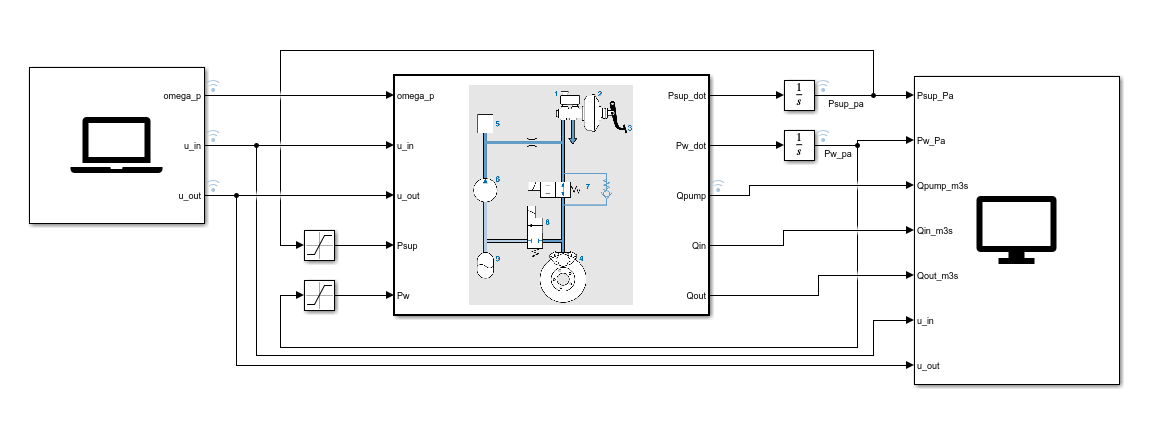
\includegraphics[width=0.8\textwidth]{figuras/image_matlab_function_bloco_hidraulico_2p.png}
    \fonte{ O Autor.}
\end{figure}

% \begin{equation}
% P_{g}(t) = \frac{P(t)-P_{ret}}{10^5}\ \ [\text{bar}].
% \label{eq:pressao_gauge_bar}
% \end{equation}

% A implementação do modelo hidráulico 2P no MATLAB Function utilizado no Simulink é apresentada no Apêndice~\ref{ap:scripts-matlab}, Código~\ref{cod:bloco_hidraulico_2p}.

%####################################################################
%####################################################################
%####################################################################
%####################################################################
\subsubsection{Teste 1: pressurização (bomba + válvula de entrada)}
\label{sec:controle-teste1}

No Teste 1, fixa-se $u_{in}=1$ e $u_{out}=0$, e aplica-se uma sequência de degraus na velocidade da bomba $\omega_p(t)$. A sequência temporal de entradas utilizada na simulação é definida no Apêndice~\ref{ap:scripts-matlab}, Código~\ref{cod:teste1_pressurizacao}.

\begin{figure}[htbp]
    \centering
    \caption{Resultado do Teste 1.}
    \label{fig:image_matlab_gerada_pelo_teste_1}
    \IfFileExists{figuras/teste1_pressurizacao.png}{%
        \includegraphics[width=0.9\textwidth]{figuras/teste1_pressurizacao.png}%
    }{%
        \fbox{\parbox{0.9\textwidth}{\centering Figura a inserir: \texttt{figuras/teste1\_pressurizacao.png}}}%
    }
    \fonte{ O Autor.}
\end{figure}

A Figura~\ref{fig:image_matlab_gerada_pelo_teste_1} apresenta o que se espera quando $P_{sup}$ e $P_w$ aumentem em patamares e que, devido à válvula de saída permanecer fechada, a pressão no canal $P_w$ tenda a se manter próxima ao patamar atingido quando $\omega_p$ retorna a zero. Esse comportamento é coerente com a presença de fluido aprisionado no volume $V_w$ na ausência de caminho de descarga e/ou vazamento equivalente.

%####################################################################
%####################################################################
%####################################################################
%####################################################################
\subsubsection{Teste 2: alívio de pressão (válvula de saída)}
\label{sec:controle-teste2}

No Teste 2, estabelece-se inicialmente um patamar de pressão (por exemplo, realizando uma etapa curta de pressurização similar ao Teste 1) e, em seguida, fixa-se $\omega_p=0$ e $u_{in}=0$, aplicando-se degraus em $u_{out}$. O roteiro temporal do ensaio e a exportação da figura são definidos no Apêndice~\ref{ap:scripts-matlab}, Código~\ref{cod:teste2_alivio_saida}.

\begin{figure}[htbp]
    \centering
    \caption{Resultado do Teste 2.}
    \label{fig:teste2_alivio_saida}
    \IfFileExists{figuras/teste2_alivio_saida.png}{%
        \includegraphics[width=0.9\textwidth]{figuras/teste2_alivio_saida.png}%
    }{%
        \fbox{\parbox{0.9\textwidth}{\centering Figura a inserir: \texttt{figuras/teste2\_alivio\_saida.png}}}%
    }
    \fonte{ O Autor.}
\end{figure}

Espera-se uma redução monotônica de $P_w$ em direção a $P_{ret}$ durante a abertura da válvula de saída, com $Q_{out}$ apresentando comportamento compatível com a lei do orifício. Em particular, quando $u_{out}$ assume valores maiores, a vazão $Q_{out}$ deve aumentar, elevando a taxa de queda de pressão no canal (maior $|\dot{P}_w|$). Caso a válvula de entrada permaneça fechada ($u_{in}=0$), o canal não recebe reposição de fluido, de modo que o comportamento dominante observado é o escoamento do volume $V_w$ para o retorno.

%####################################################################
%####################################################################
%####################################################################
%####################################################################
\subsubsection{Teste 3: restrição de entrada (variação de u\_in)}
\label{sec:controle-teste3}

No Teste 3, fixa-se $u_{out}=0$ e utiliza-se um valor constante de $\omega_p$ para manter o suprimento pressurizado, aplicando-se degraus em $u_{in}$. O roteiro temporal do ensaio e a exportação da figura são definidos no Apêndice~\ref{ap:scripts-matlab}, Código~\ref{cod:teste3_restricao_entrada}.

\begin{figure}[htbp]
    \centering
    \caption{Resultado do Teste 3.}
    \label{fig:teste3_restricao_entrada}
    \IfFileExists{figuras/teste3_restricao_entrada.png}{%
        \includegraphics[width=0.9\textwidth]{figuras/teste3_restricao_entrada.png}%
    }{%
        \fbox{\parbox{0.9\textwidth}{\centering Figura a inserir: \texttt{figuras/teste3\_restricao\_entrada.png}}}%
    }
    \fonte{ O Autor.}
\end{figure}

Este ensaio permite avaliar a influência da restrição de entrada na taxa de pressurização do canal e ajustar os parâmetros efetivos $C_{v,in}A_{in,\max}$. Espera-se que, para um mesmo patamar de $\omega_p$, aumentos em $u_{in}$ resultem em aumento de $Q_{in}$ e, consequentemente, em maior inclinação (taxa de subida) de $P_w(t)$. Como $u_{out}=0$, o crescimento de $P_w$ ocorre por transferência do suprimento para o canal; em regime, $P_w$ tende a se aproximar de $P_{sup}$ conforme o diferencial de pressão se reduz.

%####################################################################
%####################################################################
%####################################################################
%####################################################################
\subsubsection{Parâmetros iniciais e escala de vazões}
\label{sec:controle-parametros-iniciais-ensaio}

Para que os ensaios em malha aberta produzam respostas fisicamente coerentes (evitando que $Q_{in}$ seja ordens de grandeza maior do que $Q_{pump}$), os parâmetros efetivos das válvulas devem ser compatíveis com a vazão disponível da bomba no ponto de operação. Na prática, isso implica ajustar $A_{in,\max}$ e $A_{out,\max}$ de modo que $Q_{in}$ e $Q_{out}$ tenham a mesma ordem de grandeza de $Q_{pump}$ durante os degraus de $\omega_p$. Nesta pesquisa, os testes iniciais mostraram coerência ao utilizar áreas efetivas reduzidas (por exemplo, $A_{in,\max}=A_{out,\max}=10^{-7}\ \text{m}^2$) como ponto de partida, com ajustes subsequentes baseados nos sinais observados.


%####################################################################
%####################################################################
%####################################################################
%####################################################################
\subsubsection{Simulação da Resposta da Pressão Hidráulica ao Sinal}
\label{sec:controle-4-1-4-1}

A simulação da evolução das pressões $P_{sup}(t)$ e $P_w(t)$ em resposta a entradas em degrau constitui uma etapa fundamental para validar a coerência física do modelo do subsistema hidráulico antes do fechamento de malha. Nesta pesquisa, o modelo em duas pressões (Seção~\ref{sec:controle-modelo-hidraulico-2p}) foi implementado em MATLAB/Simulink, com integração numérica realizada pelo solver \texttt{ode15s}.

As entradas do ensaio são definidas como sequências temporais para a velocidade da bomba $\omega_p(t)$ e para as aberturas hidráulicas efetivas $u_{in}(t)$ e $u_{out}(t)$. As saídas analisadas incluem as pressões $P_{sup}(t)$ e $P_w(t)$, bem como as vazões internas $Q_{pump}(t)$, $Q_{in}(t)$ e $Q_{out}(t)$. Para facilitar a interpretação, as pressões são apresentadas como pressão \textit{gauge} em bar, conforme \eqref{eq:pressao_gauge_bar}.

A Figura~\ref{fig:ensaio_malha_aberta_versaoA} apresenta um resultado representativo de ensaio em malha aberta (versão didática), composto por três fases: (i) pressurização (bomba ativa e válvula de entrada aberta), (ii) retenção (válvulas fechadas, mantendo o fluido aprisionado no volume do canal), e (iii) alívio (válvula de saída aberta). Esse tipo de ensaio fornece uma base objetiva para calibração de parâmetros (por exemplo, áreas efetivas e vazamentos equivalentes) e para verificação de causalidade (crescimento/queda de pressão compatíveis com as vazões internas).

O script MATLAB utilizado para executar a simulação no Simulink e exportar esta figura (arquivo \texttt{figuras/ensaio\_malha\_aberta\_versaoA.pdf}) encontra-se no Apêndice~\ref{ap:scripts-matlab}, Código~\ref{cod:simulacao_versao_a_segura_didatica}.

\begin{figure}[htbp]
    \centering
    \caption{Ensaio em malha aberta do subsistema hidráulico (entradas, pressões e vazões).}
    \label{fig:ensaio_malha_aberta_versaoA}
    % Arquivo exportado do MATLAB (PDF/PNG). Mantém compilação mesmo se o arquivo ainda não tiver sido adicionado.
    \IfFileExists{figuras/ensaio_malha_aberta_versaoA.pdf}{%
        \includegraphics[width=0.9\textwidth]{figuras/ensaio_malha_aberta_versaoA.pdf}%
    }{%
        \fbox{\parbox{0.9\textwidth}{\centering Figura a inserir: \texttt{figuras/ensaio\_malha\_aberta\_versaoA.pdf}}}%
    }
    \fonte{ O Autor.}
\end{figure}


%####################################################################
%####################################################################
%####################################################################
%####################################################################



%####################################################################
%####################################################################
%####################################################################
%####################################################################
\section{Discussão Crítica} 
\label{cap:discussao_critica}

O desenvolvimento de um sistema de controle digital embarcado para o freio veicular com ACC representa um avanço relevante na interface entre teoria de controle, eletrônica embarcada e segurança automotiva. Contudo, como em todo projeto aplicado, é fundamental analisar criticamente as premissas, simplificações e limitações inerentes à abordagem adotada.

A modelagem do subsistema hidráulico, ainda que fundamentada em referências consolidadas, parte do pressuposto de linearidade em torno de pontos de operação e desconsidera efeitos não lineares mais complexos, como histerese das válvulas, variações térmicas do fluido, atrasos eletromecânicos e a evolução do coeficiente de atrito das lonas de freio.

Já estudos recentes sugerem que a consideração dinâmica desse coeficiente pode aprimorar a precisão da estimação da pressão de frenagem, especialmente em sistemas sujeitos a desgaste e variações operacionais \cite{ZhangWang2021}. Além disso, pesquisas sobre o projeto paramétrico de motores em sistemas de freio eletro-hidráulicos reforçam a importância de integrar modelagem precisa e validação experimental para garantir desempenho otimizado em aplicações reais \cite{MotorParametricDesign2023}. Essas simplificações foram necessárias para viabilizar a implementação em tempo real no microcontrolador automotivo, mas restringem a precisão do modelo em situações extremas ou sob condições operacionais variáveis.

Outro aspecto relevante é a ausência de validação em hardware real. Embora as simulações em MATLAB/Simulink tenham demonstrado a coerência do modelo e a viabilidade do controle, a transição para um ambiente físico envolve desafios adicionais, como latência de sensores, ruído eletromagnético, tolerâncias de fabricação e falhas intermitentes. A integração com sensores reais, como radar e câmera do sistema ADAS, também não foi abordada nesta etapa, embora seja fundamental para a operação completa do ACC.

A arquitetura modular proposta, com separação clara entre controle de alto nível ACC e controle de baixo nível (pressão hidráulica), mostrou-se alinhada com práticas contemporâneas de engenharia de sistemas embarcados. Essa modularidade facilita a substituição de blocos por versões mais sofisticadas, como controladores preditivos MPC, técnicas de controle robusto ou observadores não lineares, sem comprometer a estrutura do sistema. Além disso, a adoção de plataformas HIL pode ser considerada para validação experimental mais abrangente, aproximando ainda mais o estudo das condições reais de operação.

%####################################################################
%####################################################################
%####################################################################
%####################################################################

%####################################################################
%####################################################################
%####################################################################
%####################################################################
% \subsection{Linearização do modelo hidráulico em duas pressões}
% \label{sec:controle-linearizacao-2p}

% O modelo hidráulico em duas pressões apresentado na Seção~\ref{sec:controle-modelo-hidraulico-2p} é intrinsecamente não linear, em virtude da presença de termos de raiz quadrada nas leis de orifício das válvulas e de possíveis saturações nas diferenças de pressão. Para o projeto de controladores em espaço de estados do tipo LQR e de observadores de Luenberger, é conveniente dispor de uma aproximação linear do modelo em torno de um ponto de operação representativo.

% Neste trabalho, considera-se como vetor de estados
% \[
%     x(t) = 
%     \begin{bmatrix}
%         P_{sup}(t) \\
%         P_{w}(t)
%     \end{bmatrix},
% \]
% como vetor de entradas
% \[
%     u(t) = 
%     \begin{bmatrix}
%         \omega_p(t) \\
%         u_{in}(t) \\
%         u_{out}(t)
%     \end{bmatrix},
% \]
% e como saída de interesse a pressão no canal da roda,
% \[
%     y(t) = P_w(t).
% \]
% As equações de estado podem ser escritas de forma compacta como
% \[
%     \dot{x}(t) = f\big(x(t),u(t)\big),
% \]
% em que $f(\cdot)$ representa as relações definidas nas equações de continuidade \eqref{eq:psup_dot}–\eqref{eq:pw_dot} e nas expressões de vazão da bomba e das válvulas \eqref{eq:qpump_2p}, \eqref{eq:controle-Qin} e \eqref{eq:controle-Qout}.

% Para obter uma representação linear, adota-se a aproximação clássica por linearização em torno de um ponto de operação $(x_0,u_0)$, escolhido de forma a refletir uma condição de alta pressão de frenagem coerente com os ensaios ``realistas'' descritos na Seção~\ref{sec:controle-ajuste-parametros-realistas}. Em particular, considera-se um ponto de operação com $P_{sup}$ e $P_w$ na faixa de 50–60~bar e entradas constantes $\omega_p$, $u_{in}$ e $u_{out}$ correspondentes a uma situação de pressurização mantida (bomba acionada, válvula de entrada aberta e válvula de saída fechada).

% A linearização é realizada numericamente por meio de diferenças finitas, calculando-se as derivadas parciais de $f(x,u)$ em relação às componentes de $x$ e $u$ em torno de $(x_0,u_0)$. Em termos matriciais, obtém-se
% \[
%     \dot{\tilde{x}}(t) = A\,\tilde{x}(t) + B\,\tilde{u}(t),
%     \qquad
%     \tilde{y}(t) = C\,\tilde{x}(t) + D\,\tilde{u}(t),
% \]
% em que
% \[
%     \tilde{x}(t) = x(t) - x_0, \qquad
%     \tilde{u}(t) = u(t) - u_0,
% \]
% e as matrizes $A$ e $B$ são dadas aproximadamente por
% \[
%     A \approx \left.\frac{\partial f}{\partial x}\right|_{x_0,u_0}, 
%     \qquad 
%     B \approx \left.\frac{\partial f}{\partial u}\right|_{x_0,u_0}.
% \]

% Na implementação numérica, essas derivadas foram estimadas por diferenças finitas, perturbando-se cada componente de $x$ e $u$ em torno de $(x_0,u_0)$ e avaliando-se a variação correspondente em $\dot{x}$. O procedimento está descrito no código MATLAB \texttt{lineariza\_2P\_real.m}, apresentado no Apêndice~\ref{ap:scripts-matlab}. A partir desse código, foram obtidas as matrizes $A$ e $B$, bem como a definição de
% \[
%     C = \begin{bmatrix} 0 & 1 \end{bmatrix}, \qquad
%     D = \begin{bmatrix} 0 & 0 & 0 \end{bmatrix},
% \]
% uma vez que a saída de interesse no contexto de controle é a pressão no canal da roda $P_w$.

% Essa representação linearizada do modelo hidráulico em duas pressões será utilizada nas seções seguintes para a síntese de um regulador linear quadrático (LQR) e de um observador de Luenberger, permitindo o projeto de controladores de pressão em espaço de estados sobre uma planta que, embora simplificada, preserva as principais características dinâmicas do subsistema de freio.


%####################################################################
%####################################################################
%####################################################################
%####################################################################
% \subsection{Linearização do modelo hidráulico em duas pressões}
% \label{sec:controle-linearizacao-2p}

% Conforme apresentado na Seção~\ref{sec:controle-modelo-hidraulico-2p}, o subsistema hidráulico de freio é descrito por um modelo em duas pressões com dinâmica dada por
% \[
%     \dot{P}_{sup} = \frac{\beta}{V_{sup}}\big(Q_{pump} - Q_{in}\big), 
%     \qquad
%     \dot{P}_{w}   = \frac{\beta}{V_{w}}\big(Q_{in} - Q_{out}\big),
% \]
% em que $Q_{pump}$, $Q_{in}$ e $Q_{out}$ são as vazões da bomba, da válvula de entrada e da válvula de saída, respectivamente. No caso realista considerado (Seção~\ref{sec:controle-ajuste-parametros-realistas}), essas vazões são modeladas por
% \[
%     Q_{pump} = K_b\,\omega_p - K_{lb}\big(P_{sup} - P_{ret}\big),
% \]
% \[
%     Q_{in} = C_{v,in} A_{in,\max} u_{in}
%              \sqrt{\frac{2\big(P_{sup} - P_{w}\big)}{\rho}},
%     \qquad
%     Q_{out} = C_{v,out} A_{out,\max} u_{out}
%              \sqrt{\frac{2\big(P_{w} - P_{ret}\big)}{\rho}},
% \]
% assumindo-se que $P_{sup} > P_{w} > P_{ret}$ no ponto de operação considerado, de modo que os argumentos das funções raiz quadrada sejam positivos.

% Para fins de projeto de controladores em espaço de estados, é conveniente dispor de uma aproximação linear do modelo em torno de um ponto de operação $(x_0,u_0)$. Define-se o vetor de estados como
% \[
%     x(t) = 
%     \begin{bmatrix}
%         P_{sup}(t) \\
%         P_{w}(t)
%     \end{bmatrix},
% \]
% e o vetor de entradas como
% \[
%     u(t) = 
%     \begin{bmatrix}
%         \omega_p(t) \\
%         u_{in}(t) \\
%         u_{out}(t)
%     \end{bmatrix}.
% \]
% As equações não lineares podem ser escritas de forma compacta como
% \[
%     \dot{x}(t) = f\big(x(t),u(t)\big),
% \]
% em que $f(\cdot)$ agrega as expressões de $\dot{P}_{sup}$ e $\dot{P}_{w}$ em função de $x$ e $u$.

% A linearização em torno de $(x_0,u_0)$ é obtida pela expansão de primeira ordem de $f(x,u)$, resultando na aproximação
% \[
%     \dot{\tilde{x}}(t) \approx A\,\tilde{x}(t) + B\,\tilde{u}(t),
% \]
% em que
% \[
%     \tilde{x}(t) = x(t) - x_0, \qquad
%     \tilde{u}(t) = u(t) - u_0,
% \]
% e as matrizes $A$ e $B$ são dadas, idealmente, pelas derivadas parciais de $f$ avaliadas no ponto de operação:
% \[
%     A = \left.\frac{\partial f}{\partial x}\right|_{x_0,u_0},
%     \qquad
%     B = \left.\frac{\partial f}{\partial u}\right|_{x_0,u_0}.
% \]

% No presente trabalho, essas derivadas foram calculadas de forma analítica utilizando a \emph{Symbolic Math Toolbox} do MATLAB. Inicialmente, definiram-se simbolicamente as variáveis de estado ($P_{sup}$, $P_w$), de entrada ($\omega_p$, $u_{in}$, $u_{out}$) e os parâmetros do modelo ($\beta$, $V_{sup}$, $V_{w}$, $\rho$, $P_{ret}$, $K_b$, $K_{lb}$, $C_{v,in}$, $A_{in,\max}$, $C_{v,out}$, $A_{out,\max}$). Em seguida, foram construídas simbolicamente as expressões de $Q_{pump}$, $Q_{in}$, $Q_{out}$ e dos termos $\dot{P}_{sup}$ e $\dot{P}_{w}$, agrupando-as no vetor
% \[
%     f(x,u) = 
%     \begin{bmatrix}
%         \dot{P}_{sup} \\
%         \dot{P}_{w}
%     \end{bmatrix}.
% \]

% A partir dessa definição, as matrizes de derivadas parciais simbólicas (\emph{jacobianas}) em relação aos estados e às entradas foram determinadas por
% \[
%     A_{\text{sym}} = \frac{\partial f}{\partial x},
%     \qquad
%     B_{\text{sym}} = \frac{\partial f}{\partial u}.
% \]

% Escolheu-se então um ponto de operação $(x_0,u_0)$ representativo de uma situação de frenagem com pressão elevada, com $P_{sup}$ e $P_{w}$ na ordem de dezenas de bar e entradas constantes $\omega_p$, $u_{in}$ e $u_{out}$ compatíveis com o ensaio integrado em malha aberta realista (Seção~\ref{sec:controle-ajuste-parametros-realistas}). Os valores numéricos desse ponto e dos parâmetros físicos foram reunidos em uma estrutura (listada no código MATLAB correspondente), e as jacobianas simbólicas $A_{\text{sym}}$ e $B_{\text{sym}}$ foram avaliadas em $(x_0,u_0)$ por meio do comando \texttt{subs}, seguido da conversão para forma numérica com \texttt{double}. Dessa forma, obtiveram-se as matrizes $A$ e $B$ em forma numérica.

% A matriz de saída foi definida como
% \[
%     C = \begin{bmatrix} 0 & 1 \end{bmatrix},
% \]
% uma vez que a saída de interesse é a pressão no canal da roda $P_w$, e admitiu-se que a saída não depende diretamente das entradas no ponto de operação, de modo que
% \[
%     D = \begin{bmatrix} 0 & 0 & 0 \end{bmatrix}.
% \]

% A partir de $A$, $B$, $C$ e $D$, construiu-se o sistema linearizado em espaço de estados no MATLAB por meio do comando \texttt{ss}, o que permite tanto a análise dos polos locais do modelo (verificação de estabilidade em torno de $(x_0,u_0)$) quanto a utilização direta dessa representação em blocos do tipo \emph{State-Space} no Simulink. Essa representação linearizada constitui a base para o projeto do regulador linear quadrático (LQR) e do observador de Luenberger nas seções subsequentes.
